\subsubsection{Log Pipeline}
In the past Log engines like \gls{splunk} (\glsdesc{splunk}) were high priced data consumers, which proposed to assist in dealing with the
flow of incoming unstructured data. Without such a framework it was very hard to normalize all the data and make use of the information gathered.

In the last couple of years open-source tools emerged. The most prominent is \gls{logstash} (\glsdesc{logstash}),
followed by \gls{graylog} (\glsdesc{graylog}).
They provide a modular pipeline, which allows to take data from different inputs, normalize it (commonly in some JSON-style format)
and alter the information on the way through. Among others the data is then persisted in a data-store, e.g. in \gls{elasticsearch} (\glsdesc{elasticsearch}, see Section~\ref{elasticsearch}).
Both ecosystems provide visualization tools and connectors to a rich ecosystem.

\begin{lstlisting}[language=bash,label={lst:ls_cfg},
    caption={Example of a basic Logstash configuration which consumes events via syslog endpoint, adds a tag and writes events to stdout.}]
input {
    syslog {
        port => 5514
        type => syslog
    }
}
filter {
    mutate {
        add_tag => [ "special" ]
    }
}

output {
    stdout { codec => rubydebug }
}
\end{lstlisting}

The power of these pipelines lies in the flexibility they provide. With a couple of lines (an example is shown in \autoref{lst:ls_cfg}) of
configuration the logs are centralized and accessible via an intuitive dashboard like \gls{kibana} (\glsdesc{kibana}, see Section~\ref{kibana}) as they were never before. Compared to plain text files on each server itself this takes the accessibility of log event information to another level.

\subsubsection{Elasticsearch}
\label{elasticsearch}
Storing text in a way that allows fast searches is a complex task. Elasticsearch tackles that by pre-processing data while it is consumed by its engine.
This process is called indexing and it splits the information in various ways to speed up the search.
Elasticsearch consumes JSON formatted data and adds additional fields if needed.
If the use-case indicates that ranges in steps of hundreds are often used, the date \lstinline{value=15235} might be also stored
as \lstinline{hundred_val=15200}. This allows a binary check on the additional value instead of the evaluation of \lstinline{15200 <= 15235 and 15235 <= 15299}.

By providing use-case driven pre-processing Elasticsearch is able to provide a powerful search engine for unstructured data. Log events are a primary example in which
Elasticsearch provides fast an easy access to data.

\subsubsection{Kibana}
\label{kibana}
Kibana is an open-source javascript framework to visualize data stored in \gls{elasticsearch} (an example is shown in \autoref{fig:kibana_overview}).
\begin{figure}[!ht]
    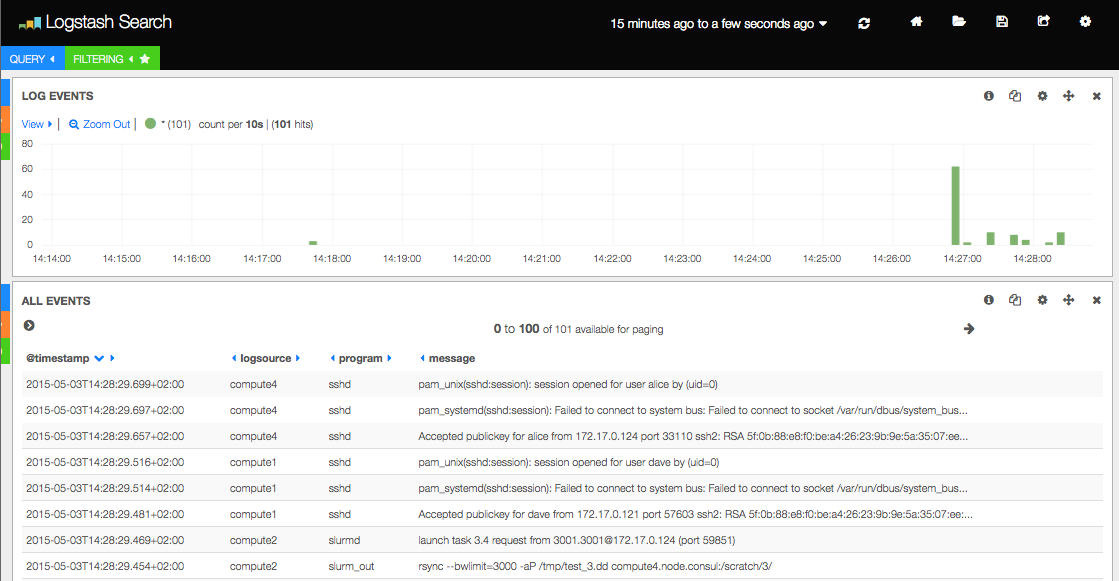
\includegraphics[width=.4\textwidth]{images/png/kibana_overview.png}
    \caption{\label{fig:kibana_overview}Example of a plain visualization of log events issued by syslog and send to Elasticsearch via Logstash.}
\end{figure}
This open source project is backed by Elastic\footnote{\Mundus~\url{https://www.elastic.co}}, the company behind Elasticsearch and integrates
seamlessly with their datastore.
